\section{Angle Between Vectors}
\label{sec:angle-between-vectors}

Having defined the \hyperref[def:length-of-a-vector]{length of a vector}, we now
turn to its \emph{direction}. Do note that direction, as well as length, can
only be defined relative to an initial value. In case of length, we use the real
numbers $0$ and $1$ for reference. In light of this, it seems apt to dedicate
some time to the study of \emph{angle} between two vectors. This way, we can say
what direction a given vector has relative to any other vectors we choose as our
initial setup. This `initial setup', we shall call a \emph{basis} in the next
chapter.

As a matter of fact, this is how we naturally specify directions when
navigating, for example. The sentence `Turn slightly right,' consists of two
messages -- one implicit and one explicit:
\begin{enumerate}
 \item Regard the direction you're facing as \emph{initial} -- forming an angle
  of $0^{ \circ }$ with your line of sight.
 \item Turn clockwise by an angle we might consider `slight', say, by $30^{
  \circ }$.
\end{enumerate}
Most of us clearly see the value in the second message and treat the first one
as obvious (ehm\dots~because it is). But, had we instead decided that the
straight line to any other surrounding point is the initial direction, step (2)
would have possibly sent us marching where no one has gone before. This benignly
intrusive introduction only served the purpose of elucidating that an initial
\emph{point of reference} is equally as important as the later specified length
or direction, despite ours taking the former for granted.

That said, this section treats all vectors as possible points of reference and
only discusses the issue of an angle of a vector relative to some other
specified vector, or said naturally, the angle between two vectors.

Dimension one being trivial -- two vectors are always collinear and can thus
only form an angle of $0^{ \circ }$ or $180^{ \circ }$ -- we start in dimension
two. Just as in the \hyperref[sec:length-of-a-vector]{previous section}, the
geometry of triangles is playing an important role here. The triangle we focus
on now is formed by three vectors: $\mathbf{v}, \mathbf{w}$ and $\mathbf{v} -
\mathbf{w}$ (cf. \myref{figure}{fig:vectors-triangle}).
\begin{figure}[ht]
 \centering
 \begin{tikzpicture}
  \tkzInit[xmin=-2,xmax=3,ymin=-1,ymax=3]
  \tkzDrawX[arrows={-Latex[width=4pt,length=6pt]},dashed,label=]
  \tkzDrawY[arrows={-Latex[width=4pt,length=6pt]},dashed,label=]
  \tkzDefPoints{1/2/a,3/1/b,0/0/O}
  \tkzMarkAngle[size=1,thick](b,O,a)
  \tkzLabelAngle[pos=0.6,yshift=.5mm](b,O,a){$\theta$}

  \tkzDrawSegment[-Latex,thick,BrickRed](O,a)
  \tkzDrawSegment[-Latex,thick,RoyalBlue](O,b)
  \tkzDrawSegment[-Latex,thick,ForestGreen](a,b)
  \tkzLabelSegment[BrickRed,above left](O,a){$\mathbf{v}$}
  \tkzLabelSegment[RoyalBlue,below=1mm](O,b){$\mathbf{w}$}
  \tkzLabelSegment[ForestGreen,above=2mm](a,b){$\mathbf{v} - \mathbf{w}$}
 \end{tikzpicture}

 \caption{The triangle defined by the vectors $\clr{\mathbf{v}}$ and
 $\clb{\mathbf{w}}$.}
 \label{fig:vectors-triangle}
\end{figure}

The properties of this triangle will allow us to calculate the angle between
$\mathbf{v}$ and $\mathbf{w}$, which we label $\theta$. The paramount ingredient
here is the \emph{Law Of Cosines}. We shall remind dear readers what it says.

\begin{theorem}{Law Of Cosines}{law-of-cosines}
 In a triangle with side lengths $a,b,c$ and angles $\alpha,\beta,\gamma$ (as in
 \myref{figure}{fig:law-of-cosines}), the following equality holds
 \[
  c^2 = a^2 + b^2 - 2ab \cos\gamma.
 \]
\end{theorem}
\begin{thmproof}
 Trivial. See, for instance, one of
 \href{https://en.wikipedia.org/wiki/Law_of_cosines#Proofs}{the many proofs on
 Wikipedia}.
\end{thmproof}

\begin{figure}[ht]
 \centering
 \begin{tikzpicture}
  \tkzDefPoints{0/0/A,2/0/B,3/3/C}
  \tkzDrawSegments(A,B A,C B,C)
  \tkzLabelSegment[below=1mm](A,B){$a$}
  \tkzLabelSegment[below right](B,C){$c$}
  \tkzLabelSegment[above left](A,C){$b$}
  \tkzMarkAngle[size=1](B,A,C)
  \tkzMarkAngle[size=0.7](C,B,A)
  \tkzMarkAngle[size=1.2](A,C,B)
  \tkzLabelAngle[pos=0.7](B,A,C){$\gamma$}
  \tkzLabelAngle[pos=0.4](C,B,A){$\beta$}
  \tkzLabelAngle[pos=0.9](A,C,B){$\alpha$}
 \end{tikzpicture}

 \caption{Auxiliary illustration to the \hyperref[thm:law-of-cosines]{Law Of
 Cosines}.}
 \label{fig:law-of-cosines}
\end{figure}

Using the \hyperref[thm:law-of-cosines]{Law Of Cosines}, we shall now proceed to
calculate the angle $\theta$ based on the entries of $\mathbf{v}$ and
$\mathbf{w}$. Substituting $a = \|\mathbf{v}\|$, $b = \|\mathbf{w}\|$ and $c =
\|\mathbf{v} - \mathbf{w}\|$ in the theorem, we get
\[
 \|\mathbf{v}-\mathbf{w}\|^2 = \|\mathbf{v}\|^2 + \|\mathbf{w}\|^2 - 2
 \|\mathbf{v}\|\|\mathbf{w}\|\cos\theta.
\]
Expanding gives
\[
 (v_1 - w_1)^2 + (v_2 - w_2)^2 = v_1^2 + v_2^2 + w_1^2 + w_2^2 - 2 \sqrt{v_1^2 +
 v_2^2}\sqrt{w_1^2 + w_2^2}\cos\theta.
\]
Now, the left side equals
\[
 (v_1^2 - w_1^2) + (v_2^2 - w_2^2) = v_1^2 - 2v_1w_1 + w_1^2 + v_2^2 - 2v_2w_2 +
 w_2^2.
\]
The squares cancel out with those on the right hand side and we reach
\[
 -2v_1w_1 - 2v_2w_2 = -2 \sqrt{v_1^2 + v_2^2}\sqrt{w_1^2 + w_2^2} \cos \theta.
\]
A final rearrangement leads to the formula for $\theta$:
\[
 \theta = \arccos \left( \frac{v_1w_1 + v_2w_2}{\sqrt{v_1^2 + v_2^2}\sqrt{w_1^2
 + w_2^2}} \right).
\]

However, this formula works only for vectors $\mathbf{v}$ and $\mathbf{w}$ of
dimension two. To proceed further, we need make an observation. The fact of the
matter is that the calculation above is almost entirely independent of the
dimensions of $\mathbf{v}$ and $\mathbf{w}$. Why? Well, the vectors $\mathbf{v}$
and $\mathbf{w}$ -- let them be $n$-dimensional -- define a two-dimensional
plane in $\R^{n}$ because each contributes one direction of movement. A good
example to make is that the vectors $\begin{psmallmatrix} 1\\ 0 \\0
\end{psmallmatrix}$ and $\begin{psmallmatrix} 0 \\1 \\0 \end{psmallmatrix}$
define the `floor' in a three-dimensional (infinite) `room' as the first one
allows horizontal movement and the second one permits moving forward and
backward. The vector $\mathbf{v} - \mathbf{w}$ lies on the same plane simply
because it's a vector rooted at the tip of $\mathbf{v}$ and ending in the tip
of $\mathbf{w}$. This means that no matter what dimension $\mathbf{v}$ and
$\mathbf{w}$ lie in, they still form the same triangle as in
\myref{figure}{fig:vectors-triangle}, which now lies on a plane in $\R^{n}$. As
a consequence, the calculation we just did is still almost valid; it only need
be upgraded to vectors with $n$ real entries.

We've just observed that for $\mathbf{v}, \mathbf{w} \in \R^{n}$ the equality
\[
 \|\mathbf{v}-\mathbf{w}\|^2 = \|\mathbf{v}\| + \|\mathbf{w}\| - 2
 \|\mathbf{v}\|\|\mathbf{w}\|\cos\theta
\]
still stands. Applying the same transformations as before, we reach the
expression for $\theta$:
\[
 \theta = \arccos \left( \frac{v_1w_1 + v_2w_2 + \ldots + v_nw_n}{\sqrt{v_1^2 +
 v_2^2 + \ldots + v_n^2}\sqrt{w_1^2 + w_2^2 + \ldots + w_n^2}} \right).
\]
The denominator of the fraction is of course simply
$\|\mathbf{v}\|\|\mathbf{w}\|$ and the nominator is the output of a function
called the \emph{dot} (or \emph{scalar}) product. It has beautiful geometric
properties and is paramount to a deeper study of linear systems but for now it
only serves the purpose of convenient notation.

\begin{definition}{Dot product}{dot-product}
 The \emph{dot product} of vectors
 \[
  \mathbf{v} =
  \begin{pmatrix}
   v_1\\
   v_2\\
   \vdots\\
   v_n
  \end{pmatrix},
  \mathbf{w} = 
  \begin{pmatrix}
   w_1\\
   w_2\\
   \vdots\\
   w_n
  \end{pmatrix} \in \R^{n}
 \]
 is defined as
 \[
  \mathbf{v} \cdot \mathbf{w} \coloneqq v_1w_1 + v_2w_2 + \ldots + v_nw_n.
 \]
\end{definition}

Note that the dot product of two vectors is a \textbf{number}, not a vector, and
it is defined only for vectors with the same number of entries. More
interestingly, it is tied to the \hyperref[def:length-of-a-vector]{length of a
vector} by the formula
\[
 \|\mathbf{v}\|^2 = \mathbf{v} \cdot \mathbf{v}.
\]
We intend to make use of this formula down the line.

There is one last problem to be solved before we can properly define the angle
between two vectors. As educated readers well know, the function $\arccos$ is
only takes input from the closed interval $[-1,1]$. Since we intend to define
$\theta$ as $\arccos(\mathbf{v} \cdot \mathbf{w} /
\|\mathbf{v}\|\|\mathbf{w}\|)$, we must make sure that the argument is always in
said interval.

We actually aim to present a little stronger result the proof whereof will
contain the desired inequality. This result styles the \emph{triangle
inequality} and is the cornerstone of Euclidean geometry -- `The shortest
distance between two points is a straight line.'

\begin{figure}[ht]
 \centering
 \begin{tikzpicture}
  \tkzDefPoints{0/0/a,4/1/b,5/3/c}
  \tkzDrawSegment[-Latex,thick,BrickRed,shorten >=4pt,shorten <=4pt](a,b)
  \tkzDrawSegment[-Latex,thick,RoyalBlue,shorten >=4pt,shorten <=4pt](a,c)
  \tkzDrawSegment[-Latex,thick,ForestGreen,shorten >=4pt,shorten <=4pt](b,c)
  \tkzDrawPoints[size=6](a,b,c)
  \tkzLabelPoint[left=1mm](a){\texttt{start}}
  \tkzLabelPoint[right=1mm](c){\texttt{end}}
  \tkzLabelSegment[BrickRed,below=1mm](a,b){$\mathbf{v}$}
  \tkzLabelSegment[ForestGreen,below right](b,c){$\mathbf{w}$}
  \tkzLabelSegment[RoyalBlue,above left](a,c){$\mathbf{v} + \mathbf{w}$}
 \end{tikzpicture}

 \caption{The triangle inequality.}
 \label{fig:triangle-inequality}
\end{figure}

\begin{theorem}{Triangle inequality}{triangle-inequality}
 For any vectors $\mathbf{v},\mathbf{w} \in \R^{n}$ the inequality
 \begin{equation}
  \label{eq:triangle-inequality}
  \|\mathbf{v} + \mathbf{w}\| \leq \|\mathbf{v}\| + \|\mathbf{w}\|
 \end{equation}
 holds. Furthermore, the two sides are equal if and only if $\mathbf{v}$ is a
 scalar multiple of $\mathbf{w}$.
\end{theorem}
\begin{thmproof}
 We shall use a few properties of the \hyperref[def:dot-product]{dot product} we
 haven't proven. Namely,
 \begin{itemize}
  \item $\mathbf{u} \cdot (\mathbf{v} + \mathbf{w}) = \mathbf{u} \cdot
   \mathbf{v} + \mathbf{u} \cdot \mathbf{w}$;
  \item $\mathbf{v} \cdot \mathbf{w} = \mathbf{w} \cdot \mathbf{v}$;
 \end{itemize}
 these are left as an exercise.

 We now proceed to make a few algebraic manipulations to the
 inequality~\eqref{eq:triangle-inequality}. First, both sides are positive
 numbers, hence the inequality is equivalent to
 \[
  \|\mathbf{v} + \mathbf{w}\|^2 \leq (\|\mathbf{v}\| + \|\mathbf{w}\|)^2.
 \]
 Rewriting slightly (and using $\|\mathbf{v}\|^2 = \mathbf{v} \cdot \mathbf{v}$)
 \begin{align*}
  (\mathbf{v} + \mathbf{w}) \cdot (\mathbf{v} + \mathbf{w}) &\leq
  \|\mathbf{v}\|^2 + \|\mathbf{w}\|^2 + 2 \|\mathbf{v}\|\|\mathbf{w}\|\\
  \mathbf{v} \cdot \mathbf{v} + \mathbf{v} \cdot \mathbf{w} + \mathbf{w} \cdot
  \mathbf{v} + \mathbf{w} \cdot \mathbf{w} &\leq \mathbf{v} \cdot \mathbf{v} +
  \mathbf{w} \cdot \mathbf{w} + 2 \|\mathbf{v}\|\|\mathbf{w}\|\\
  2(\mathbf{v} \cdot \mathbf{w}) & \leq 2 \|\mathbf{v}\|\|\mathbf{w}\|.
 \end{align*}
 Multiplying both sides by $\|\mathbf{v}\|\|\mathbf{w}\|$ gives
 \begin{align*}
  2 \|\mathbf{v}\|\|\mathbf{w}\|(\mathbf{v} \cdot \mathbf{w}) &\leq 2
  \|\mathbf{v}\|^2 \|\mathbf{w}\|^2\\
  2(\|\mathbf{w}\|\mathbf{v} \cdot \|\mathbf{v}\|\mathbf{w}) & \leq 2
  \|\mathbf{v}\|^2 \|\mathbf{w}\|^2,
 \end{align*}
 and further manipulation then
 \[
  0 \leq \|\mathbf{v}\|^2 \|\mathbf{w}\|^2 - 2(\|\mathbf{w}\|\mathbf{v} \cdot
  \|\mathbf{v}\|\mathbf{w}) + \|\mathbf{v}\|^2 \|\mathbf{w}\|^2.
 \]
 Finally, as
 \[
  \|\mathbf{v}\|\mathbf{w} \cdot \|\mathbf{v}\|\mathbf{w} =
  \|\mathbf{v}\|^2(\mathbf{w} \cdot \mathbf{w}) =
  \|\mathbf{v}\|^2\|\mathbf{w}\|^2 \quad \text{and} \quad
  \|\mathbf{w}\|\mathbf{v} \cdot \|\mathbf{w}\|\mathbf{v} =
  \|\mathbf{w}\|^2(\mathbf{v} \cdot \mathbf{v}) = \|\mathbf{w}\|^2
  \|\mathbf{v}\|^2,
 \]
 we can complete the square and get
 \begin{equation}
  \label{eq:triangle-inequality-square}
  0 \leq (\|\mathbf{w}\|\mathbf{v} - \|\mathbf{v}\|\mathbf{w}) \cdot
  (\|\mathbf{w}\|\mathbf{v} - \|\mathbf{v}\|\mathbf{w}) = \big\|
  \|\mathbf{w}\|\mathbf{v} - \|\mathbf{v}\|\mathbf{w} \big\|^2.
 \end{equation}
 The right hand side is the length of the vector $\|\mathbf{w}\|\mathbf{v} -
 \|\mathbf{v}\|\mathbf{w}$ squared, that is, definitely a non-negative number.
 This proves the inequality.

 As for the conditional equality statement, the
 inequality~\eqref{eq:triangle-inequality-square} suggests that the two sides of
 the original inequality~\eqref{eq:triangle-inequality} are equal if and only if
 \[
  \|\mathbf{w}\|\mathbf{v} - \|\mathbf{v}\|\mathbf{w} = 0
 \]
 but this clearly happens if and only if
 \begin{align*}
  \|\mathbf{w}\|\mathbf{v} &= \|\mathbf{v}\|\mathbf{w}\\
  \mathbf{v} &= \frac{\|\mathbf{v}\|}{\|\mathbf{w}\|}\mathbf{w},
 \end{align*}
 that is, if and only if $\mathbf{v}$ is the $(\|\mathbf{v}\| /
 \|\mathbf{w}\|)$-multiple of $\mathbf{w}$.

 This concludes the proof.
\end{thmproof}

\begin{exercise}{Some properties of dot product}{some-properties-of-dot-product}
 Prove that for any three vectors $\mathbf{u},\mathbf{v},\mathbf{w} \in \R^{n}$,
 the following equalities hold:
 \begin{itemize}
  \item $\mathbf{u} \cdot (\mathbf{v} + \mathbf{w}) = \mathbf{u} \cdot
   \mathbf{v} + \mathbf{u} \cdot \mathbf{w}$,
  \item $\mathbf{v} \cdot \mathbf{w} = \mathbf{w} \cdot \mathbf{v}$.
 \end{itemize}
\end{exercise}

As a corollary, we get the inequality which is widely remembered as the
\emph{Cauchy-Schwarz inequality} and plays an indispensable role in linear
algebra as well as other branches of mathematics, such as the theory of metric
spaces and, by extension, the theory of Lebesgue integration.

\begin{corollary}{Cauchy-Schwarz inequality}{cauchy-schwarz-inequality}
 For any $\mathbf{v},\mathbf{w} \in \R^n$, the inequality
 \[
  |\mathbf{v} \cdot \mathbf{w}| \leq \|\mathbf{v}\|\|\mathbf{w}\|
 \]
 holds and the two sides are equal if and only if $\mathbf{v}$ is a scalar
 multiple of $\mathbf{w}$.
\end{corollary}
\begin{corproof}
 The proof of \myref{theorem}{thm:triangle-inequality} suggests that
 \[
  \mathbf{v} \cdot \mathbf{w} \leq \|\mathbf{v}\|\|\mathbf{w}\|
 \]
 so if $\mathbf{v} \cdot \mathbf{w}$ is non-negative, we don't have anything to
 prove. On the other hand, if $\mathbf{v} \cdot \mathbf{w}$ is negative, we
 compute
 \[
  |\mathbf{v} \cdot \mathbf{w}| = -(\mathbf{v} \cdot \mathbf{w}) =
  (-\mathbf{v}) \cdot \mathbf{w} \leq \|-\mathbf{v}\|\|\mathbf{w}\| =
  \|\mathbf{v}\|\|\mathbf{w}\|
 \]
 and we're done.
\end{corproof}

We've reached the end of the section where we finally properly define the angle
between two vectors. This definition is justified by the last
\myref{corollary}{cor:cauchy-schwarz-inequality} since it assures that
\[
 \frac{\mathbf{v} \cdot \mathbf{w}}{\|\mathbf{v}\|\|\mathbf{w}\|} \in [-1,1]
\]
and so the real number
\[
 \arccos \left( \frac{\mathbf{v} \cdot \mathbf{w}}{\|\mathbf{v}\|\|\mathbf{w}\|}
 \right)
\]
exists for all vectors $\mathbf{v},\mathbf{w} \in \R^{n}$.

\begin{definition}{Angle between vectors}{angle-between-vectors}
 For any $\mathbf{v},\mathbf{w} \in \R^{n}$, we define the angle $\theta$
 between $\mathbf{v}$ and $\mathbf{w}$ as the number
 \[
  \theta = \arccos \left( \frac{\mathbf{v} \cdot
  \mathbf{w}}{\|\mathbf{v}\|\|\mathbf{w}\|} \right).
 \]
\end{definition}
